\documentclass{beamer}
\usepackage{ragged2e}
\usepackage[frenchb]{babel}
\usetheme[subsectionpage=progressbar]{metropolis}
\usepackage{fancyvrb}
\usepackage{graphicx}
\usepackage{listings}
\usepackage{xcolor}

\setcounter{tocdepth}{1}
\apptocmd{\frame}{}{\justifying}{} % Allow optional arguments after frame.

\colorlet{punct}{red!60!black}
\definecolor{background}{HTML}{EEEEEE}
\definecolor{delim}{RGB}{20,105,176}
\colorlet{numb}{magenta!60!black}

\lstdefinelanguage{json}{
  basicstyle=\normalfont\ttfamily,
  numbers=left,
  numberstyle=\scriptsize,
  stepnumber=1,
  numbersep=8pt,
  showstringspaces=false,
  breaklines=true,
  frame=lines,
  backgroundcolor=\color{background},
  literate=
  *{0}{{{\color{numb}0}}}{1}
  {1}{{{\color{numb}1}}}{1}
  {2}{{{\color{numb}2}}}{1}
  {3}{{{\color{numb}3}}}{1}
  {4}{{{\color{numb}4}}}{1}
  {5}{{{\color{numb}5}}}{1}
  {6}{{{\color{numb}6}}}{1}
  {7}{{{\color{numb}7}}}{1}
  {8}{{{\color{numb}8}}}{1}
  {9}{{{\color{numb}9}}}{1}
  {:}{{{\color{punct}{:}}}}{1}
  {,}{{{\color{punct}{,}}}}{1}
  {\{}{{{\color{delim}{\{}}}}{1}
  {\}}{{{\color{delim}{\}}}}}{1}
  {[}{{{\color{delim}{[}}}}{1}
  {]}{{{\color{delim}{]}}}}{1},
}

\title{MVC, Composer, Laravel}
\date{}
\author{Lionel \textsc{Kitihoun}}

\begin{document}
\begin{frame}[plain]
\maketitle
\end{frame}

\begin{frame}{Sommaire}
\tableofcontents
\end{frame}

\section{MVC}
\begin{frame}{MVC}
  Patron de conception qui met en avant la séparation du code des applications en trois éléments :
  \begin{itemize}
    \item Le modèle, qui représente les données manipulées et les traitements métier associés.
    \item La vue, l'interface de l'application avec laquelle l'utilisateur interagit.
    \item Le contrôleur, qui détermine les traitements à éffectuer en fonctions des actions de l'utilisateur.
  \end{itemize}
\end{frame}

\begin{frame}{Modèle de fonctionnement}
  \begin{center}
    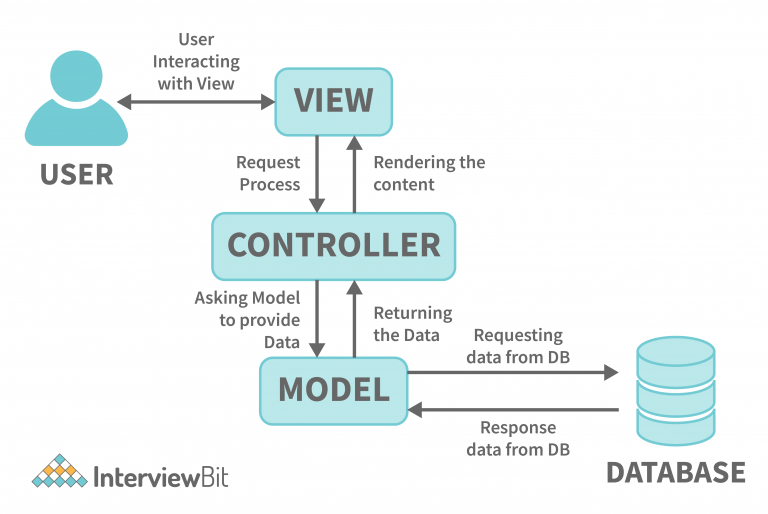
\includegraphics[scale=0.4]{images/working-of-mvc.png}
  \end{center}
\end{frame}

\begin{frame}{Origines et utilisation actuelle du MVC}
  Le MVC a été créé pour faciliter le développement des applications graphiques. Il est par exemple utilisé par Swing et Qt.
  
  Mais il a été appliqué avec succès dans le domaines des applications web car il facilite grandement le processus de développement et permet le partage des tâches entre les devs.
\end{frame}

\begin{frame}{Modèle de fonctionnement (Web) I}
  \begin{center}
    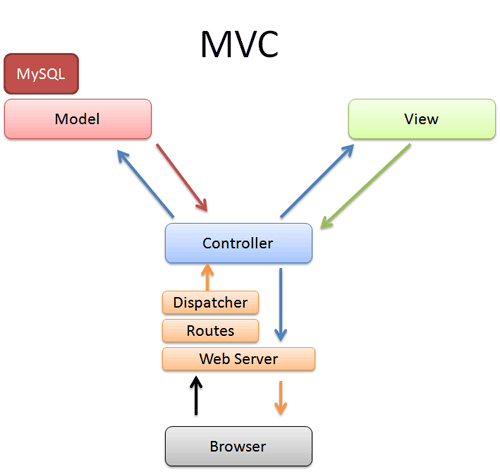
\includegraphics[scale=0.3]{images/mvc-rails.converted.png}
  \end{center}
\end{frame}

\begin{frame}{Modèle de fonctionnement (Web) II}
  \begin{center}
    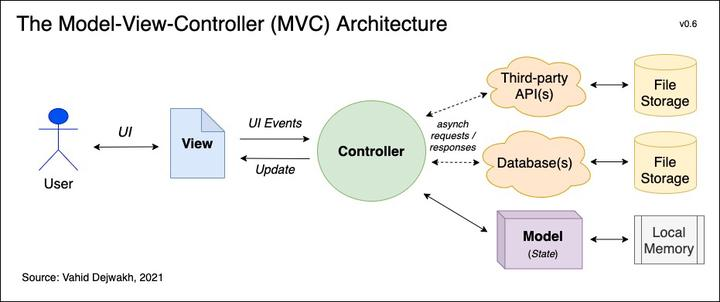
\includegraphics[scale=0.4]{images/mvc-architecture.jpg}
  \end{center}
\end{frame}

\begin{frame}{Frameworks MVC}
  \begin{itemize}
    \item PHP : Laravel, Symfony.
    \item Python : Django.
    \item Ruby : Ruby on Rails.
    \item Java : Spring.
  \end{itemize}
\end{frame}

\section{Composer}
\begin{frame}{Composer}
\begin{center}
  
\includegraphics[scale=1.5]{images/composer.png}
\end{center}
\end{frame}

\begin{frame}{Composer}
\begin{itemize}
  \item Gestionnaire de dépendances pour les projets PHP.
  \item Inspiré de NPM (Node Package Manager).
  \item Installe les paquets depuis \url{https://packagist.org/}.
\end{itemize}
\end{frame}

\begin{frame}[fragile]
\frametitle{Utilisation I}
  1. Déclarer les dépendances dans un fichier \texttt{composer.json} à la racine du projet.
  \begin{lstlisting}[language=json]
    {
      "require": {
        "psr/log": "1.3.2",
        "fakerphp/faker": "1.*",
        "guzzlehttp/guzzle": "^7.4.0"
      }
    }
  \end{lstlisting}
\end{frame}

\begin{frame}{Utilisation II}
  2. Installer Composer (globalement ou en local).
\end{frame}

\begin{frame}[fragile]{Utilisation III}
  3. Installer les paquets avec la commande :
  \begin{Verbatim}
    php composer.phar install # Installation locale
    composer install # Installation globale
  \end{Verbatim}
\end{frame}

\begin{frame}[fragile]{Utilisation IV}
  4. Charger automatiquement les dépendances à l'exécution avec l'instruction :
  \begin{verbatim}
    require 'vendor/autoload.php';
  \end{verbatim}
\end{frame}

\section{Laravel}
\begin{frame}{Laravel}
\begin{itemize}
  \item Framework MVC écrit en PHP très populaire.
  \item \url{https://laravel.com}
    \vspace{10pt}
    \begin{center}
      
\includegraphics[scale=0.3]{images/laravel.png}
    \end{center}
\end{itemize}
\end{frame}

\begin{frame}[fragile]
\frametitle{Création d'un projet avec Composer}
\begin{Verbatim}[fontsize=\scriptsize]
  composer create-project --prefer-dist laravel/laravel my-project
\end{Verbatim}
\end{frame}

\begin{frame}[fragile]
\frametitle{Création d'un projet à version spécifique}
\begin{center}
\begin{Verbatim}[fontsize=\scriptsize]
composer create-project --prefer-dist laravel/laravel getting-started 9.5
\end{Verbatim}
\end{center}
\end{frame}

\begin{frame}[fragile]
\frametitle{Création d'un projet avec l'installeur Laravel}
\begin{Verbatim}[fontsize=\small]
  composer global require laravel/installer
  laravel new my-super-project
\end{Verbatim}
\end{frame}

\begin{frame}{Page d'accueil par défaut}
\begin{center}
  
\includegraphics[scale=0.25]{images/laravel-welcome-page.png}
\end{center}
\end{frame}
\end{document}
